Drei Körper mit den Massen $m_1 = \mSaO$, $m_2 = \mSbO$ und $m_3 = \mScO$ sind an einem Stab befestigt ($a = \aSpO$, $b = \bSpO$). Wie weit ist der Schwerpunkt von $m_1$ entfernt? Die Masse des Stabes sei vernachlässigbar.

\begin{center}
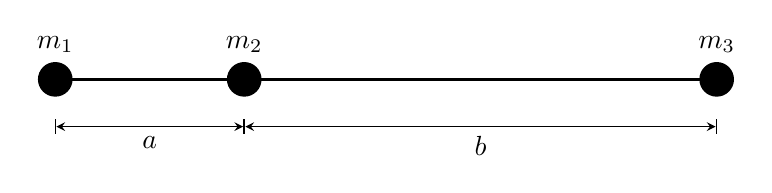
\begin{tikzpicture}[>=stealth]
 \draw[very thick] (0,0) -- (8.4,0);
 \fill (0,0) circle (0.22) node[above=6pt] {$m_1$};
 \fill (2.4,0) circle (0.22) node[above=6pt] {$m_2$};
 \fill (8.4,0) circle (0.22) node[above=6pt] {$m_3$};
 \draw[|<->|] (0,-0.6) -- (2.4,-0.6) node[midway, below] {$a$};
 \draw[|<->|] (2.4,-0.6) -- (8.4,-0.6) node[midway, below] {$b$};
\end{tikzpicture}
\end{center}
